
%        File: HW**_Last_First.tex
%     Created: Fri Aug 07 04:00 PM 2015 M
% Last Change: Fri Aug 07 04:00 PM 2015 M
%
\documentclass[a4paper]{article}
\usepackage[table]{xcolor}
\usepackage{amsmath,amsthm,amsfonts}
\usepackage{tikz,pgfplots}
\usepackage{graphicx}
\usepackage[margin=1.75cm]{geometry}
\usepackage{setspace}
\usepackage{multirow}
\usepackage{float}
\makeatletter
\newcommand*\bigcdot{\mathpalette\bigcdot@{.5}}
\newcommand*\bigcdot@[2]{\mathbin{\vcenter{\hbox{\scalebox{#2}{$\m@th#1\bullet$}}}}}
\makeatother


\newcommand\abs[1]{\left|#1\right|}
\newcommand{\doubleunderline}[1]{\underline{\underline{#1}}}
\onehalfspacing
\allowdisplaybreaks

\usepackage[colorlinks]{hyperref}

\theoremstyle{remark}
\newtheorem*{solution}{Solution}

\theoremstyle{remark}
\newtheorem*{example}{Example}



\title{Modeling Contaminant Flow in the Puget Sound\\}
\author{Jordan Trinka\\
Advisor: Eric Sullivan Ph.D.}
\date{\today}


\usepackage{fancyhdr}
 

\pagestyle{fancy}
\fancyhf{}
\rhead{Trinka}
\lhead{}

\begin{document}
\maketitle
\begin{abstract}
Oil spills in large bodies of water cause severe complications and damages in aquatic ecosystems. Being able to predict what areas of an aquatic ecosystem would be most damaged by an oil spill would prove to be invaluable in shortening clean up time, easing clean up effort, and saving more of the environment. For this reason, we will mathematically model contaminant flow in an aquatic domain to try to predict what areas of the ecosystem will be most effected by a spill. We will consider predicting contaminant flow in a two-dimensional domain model of the Puget Sound by a numerical solution to the advection-diffusion equation coupled with the Navier-Stokes equations. We will offer two models of contaminant flow in this domain, the first will be a Gaussian point source model of contaminant flow which will simulate a ship going down in the Sound with a leak that spreads in a uniform circular form. The second model of contaminant flow will be of a constant source leak into the Puget Sound from along the shoreline to model a pipeline is leaking into the Sound. We will solve the advection-diffusion equation using a finite element method and the Navier-Stokes equations with a finite difference method.
\end{abstract}

\newpage
\lhead{Contents}
\tableofcontents % This line creates the table of contents (DO NOT CHANGE)
\vspace{0.1in}\hrule
\newpage
\lhead{List of Figures and List of Tables}
\listoffigures
\listoftables
\newpage
\lhead{}

\section{Introduction} \label{intro}
The Deepwater Horizon spill of April, 2010 was a massive environmental catastrophe that damaged much of the ecosystem of the Gulf of Mexico. This spill prompted an intense clean up effort by volunteers, government environmental agencies, and the United States Navy. Effected areas needed to be located, contained, and cleaned up. Figuring out what areas would be most contaminated and thus would be most effected before the spill would help clean up crews pinpoint what areas would require the most attention prior to the spill. The goal of this paper is to mathematically model the advection and diffusion of oil on the surface of a body of water by a finite element numerical solution to the advection-diffusion equation in order to predict what areas of an environment would be most damaged by a spill. To solve the advection-diffusion equation, we also need a velocity vector field which we will solve for using a finite difference numerical solution to the Navier-Stokes equations. We will use these approximate solutions to create two models of an oil spill in the Puget Sound when water is flowing out. One model will consist of a point source model of a sinking ship and the other will model a constant source spill into the domain from a broken pipeline.
\par
We will start by giving an introduction into the finite element method in section \ref{OverviewFEM} by numerically solving a second order, non-homogeneous, ordinary differential equation. We will then show our Puget Sound domain in which we wish to model contaminant flow on and offer our treatment of boundary conditions for the two models in section \ref{DomainSection}. After this we will discuss our methods which were used to solve the advection-diffusion equation numerically as well as our Navier-Stokes velocity vector field which we cover in sections \ref{AdvecDiffSec} and \ref{Navier-Stokes section}. We then offer our results that we obtain from our two models in section \ref{Results Section} and perform a sensitivity analysis on both models which can be found in section \ref{SensitivityAnalysisSection}. We finish with a discussion of future work in section \ref{futureworksection} and a conclusion in section \ref{conclusionsection}.
%Discuss what's coming

\section{Overview of the Finite Element Method} \label{OverviewFEM}
%Talk to Dr. Sullivan
The purpose of using the finite element method is to be able to approximate the solution to boundary value problems. In particular, the finite element method is often employed to numerically solve partial differential equations on complex domains where an ``analytic solution is not readily available" \cite{Sullivan}. We will summarize a problem that is solved in \cite{Johnson} in order to introduce the reader to the finite element method. All work in the rest of this section is drawn from \cite{Johnson} and \cite{50LinesofMATLAB}. Consider the following

\begin{equation}\label{testfem1}
-u'' \left(x \right)=f\left(x \right)
\end{equation}
where $u \in H^{1}\left(\Omega \right)$, $u\left(0 \right) = u\left(1 \right) = 0$ for $0<x<1$ which is our domain $\Omega$. The space $H^{1}$ is a Sobolev space which contains functions with enough derivatives which can be applied to some domain. By integrating twice, we find there is an analytic solution $u(x)$, however, for purposes of this quick overview, we will solve \eqref{testfem1} numerically by the finite element method. We start by getting the weak form of \eqref{testfem1} by multiplying both sides by a test function $v\in H^{1}\left(\Omega \right)$ and integrating both sides to get

\begin{equation}\label{testfem2}
\int_{\Omega} -u'' \left(x \right) v\left(x \right) dx=\int_{\Omega} f\left(x \right) v\left(x \right) dx
\end{equation}

\noindent We integrate the left-hand side of \eqref{testfem2} by parts and use the fact that $u\left(0 \right) = u\left(1 \right) = 0$ to get

\begin{equation}\label{testfem3}
\int_{\Omega} u' \left(x \right) v'\left(x \right) dx=\int_{\Omega} f\left(x \right) v\left(x \right) dx.
\end{equation}

\noindent Next we create a finite set of nodes $j$ along $\Omega$ which we will use to interpolate \eqref{testfem3} at each $j$. In doing this, we also construct the following set of basis functions
%illustration

$$
\phi_{i}\left(x_{j} \right)=
\begin{cases}
1 \texttt{ if } i=j,\\
0 \texttt{ if } i\neq j, \texttt{ for } i,j=1,...,M
\end{cases}
$$
%discuss with Sullivan
where $M$ is the maximum number of nodes which we specified along $\Omega$. Notice that these basis functions create a set of linear, affine, triangular regions of $\Omega$ \cite{50LinesofMATLAB}. From here, we can write $u\left(x\right)$ and $v\left(x\right)$ as a finite dimensional linear combination of the basis functions $\phi_{j}$ \cite{Sullivan} as shown below
\begin{eqnarray}\label{UVdiscrete}
v\left(x \right) &=& \sum_{i=1}^{M} \eta_{i} \phi_{i}\left(x_{i} \right)\\
\nonumber
u\left(x \right) &=& \sum_{j=1}^{M} \xi_{j} \phi_{j}\left(x_{j} \right).
\end{eqnarray}
where $x \in [0,1]$, $\eta_{i}=v\left(x_{i}\right)$, and $\xi_{j}=u\left(x_{j}\right)$. Using these interpolations, we see that \ref{testfem3} becomes

\begin{equation}\label{testfem4}
\sum_{i=1}^{M}\xi_{j}\int_{\Omega} \phi_{j}'\phi_{i}'dx=\sum_{i=1}^{M} \int_{\Omega} f\left(x_{i}\right)\phi_{i}dx, j=1,...,M.
\end{equation}

\noindent This is a linear system of the form 
\begin{equation}\label{testfem5}
\mathbf{A}\underline{\xi}=\underline{b}.
\end{equation}

\noindent From here we define $\mathbf{A}=\sum_{i=1}^{M}\int_{\Omega} \phi_{i}'\phi_{j}'dx$ and $\underline{b}=\sum_{i=1}^{M} \int_{\Omega} f\left(x_{i}\right)\phi_{i}dx$.
We can compute the elements $\mathbf{A}$ by first noticing that $\phi_{j}'\phi_{i}'=0$ if $\abs{i-j}>1 \texttt{ } \forall \texttt{ } x\in [0,1]$. This fact causes $\mathbf{A}$ to be tri-diagonal. We have for $j=1,...,M$

\begin{equation} \label{testfem6}
\int_{\Omega} \phi_{j}'\phi_{j}'dx=\int_{x_{j-1}}^{x_{j}} \frac{1}{h_{j}^{2}}dx+\int_{x_{j}}^{x_{j+1}} \frac{1}{h_{j+1}^{2}}dx = \frac{1}{h_{j}}+\frac{1}{h_{j+1}} 
\end{equation}

\noindent and for the other diagonals, we have for $j=2,...,M$

\begin{equation}
\int_{\Omega} \phi_{j}'\phi_{j-1}'dx=\int_{\Omega} \phi_{j-1}'\phi_{j}'dx=-\int_{x_{j-1}}^{x_{j}} \frac{1}{h_{j}^{2}}dx=-\frac{1}{h_{j}} 
\end{equation}

\noindent If we partition our domain uniformly with $h_{j}=\frac{1}{M+1}$, then \eqref{testfem5} becomes
%Talk to Sullivan
\begin{equation}\label{testfem7}
\frac{1}{h}\begin{bmatrix}
2 & -1 & 0 & . & . & . & . & . & 0\\
-1 & 2 & -1 & . & . & . & . & . & .\\
0 & -1 & 2 & -1  & . & . & . & . & .\\
. & . & . & . & . & . & . & . & .\\
. & . & . & . & . & . & . & . & .\\
. & . & . & . & . & . & . & 2 & -1\\
0 & . & . & . & . & . & . & -1 & 2
\end{bmatrix}
\begin{bmatrix}
\xi_{1}\\
.\\
.\\
.\\
.\\
.\\
\xi_{M}
\end{bmatrix}
=
\begin{bmatrix}
b_{1}\\
.\\
.\\
.\\
.\\
.\\
b_{M}
\end{bmatrix}
\end{equation}

\noindent Row reduction can be used to solve \eqref{testfem7} for $\underline{\xi}$. Now that we have an idea of how the finite element method works, we can continue into our particular problem.

\section{Puget Sound Domain, Boundary, and Initial Conditions} \label{DomainSection}
We will start with our Puget Sound domain $\Omega \subset \mathbb{R}^{2}$ where $\Omega$ is a bounded Lipschitz domain that also has a polygonal boundary $\Gamma$ \cite{50LinesofMATLAB}. Our domain is shown in Figure \ref{MyDomain} outlined in black and red.
\begin{figure}[H]\label{MyDomain}
   
\centering   
   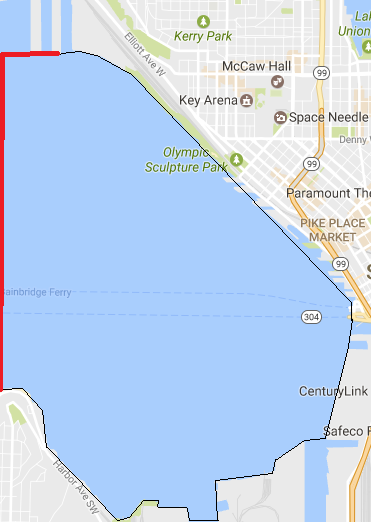
\includegraphics[width=0.4\linewidth]{domainoutline.png}
    \caption{Puget Sound Domain}
    \label{pugetsounddomain}
    %left lower right upper
\end{figure}

We will use Neumann boundary conditions $\Gamma_{\texttt{N}}$ along the boundary outlined in black while the red outlined boundary will be Dirichlet $\Gamma_{\texttt{D}}$ such that $\Gamma = \Gamma_{\texttt{N}} \cup \Gamma_{\texttt{D}}$. We will create two models of contaminant flow within $\Omega$. The first model will utilize an arbitrarily chosen point source Gaussian initial condition of contaminant with $\Gamma_{\texttt{D}}=0$ along the red boundary and $\Gamma_{\texttt{N}}=0$ along the black boundary of the domain. The second model will utilize a point source Gaussian initial condition of contaminant and a constant source of contaminant along part of $\Gamma_{\texttt{N $\rightarrow$ D}}$ in order to model a constant spill into $\Omega$ where $\Gamma_{\texttt{N $\rightarrow$ D}}$ is a portion of the Neumann boundary which will be transformed into a Dirichlet boundary resulting in non-homogeneous Dirichlet boundaries. This new boundary condition is outlined in magenta in the following figure

\begin{figure}[H]\label{MyDomain}
   
\centering   
   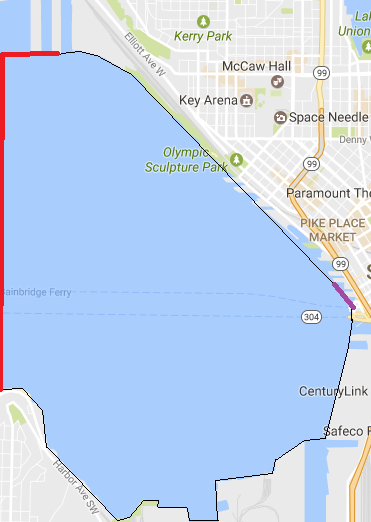
\includegraphics[width=0.4\linewidth]{domainoutline2.png}
    \caption{Puget Sound Domain with Non-Homogenous Dirichlet Conditions}
    \label{pugetsounddomain2}
    %left lower right upper
\end{figure}


\noindent We choose the value along $\Gamma_{\texttt{N $\rightarrow$ D}}$ to be close in value to that of the peak of our gaussian function with the rest of $\Gamma_{\texttt{D}}=0$. We also choose the remaining $\Gamma_{\texttt{N}}=0$.

\section{The Advection-Diffusion Equation} \label{AdvecDiffSec}
%Explain the advection diffusion equation here
Consider the advection-diffusion equation
\begin{equation} \label{advecdiff}
\frac{\partial u}{\partial t} = D\Delta u + \underline{v} \bigcdot \underline{\nabla}u+f
\end{equation}
where $f \in L^{2}\left(\Omega\right)$, $u,v \in H^{1}\left(\Omega\right)$, $\Delta$ is the Laplace operator, and $L^{2}$ is the space that contains all square integrable functions \cite{Sullivan}.
We see that the left-hand side of \eqref{advecdiff} is the change in concentration of contaminant with respect to time, $\Delta u$ models the diffusion of contaminant, $\underline{v} \bigcdot \underline{\nabla}u$ models the advection of contaminant, and $f$ is a forcing term.
For purposes of this project, we take $t$ to be time measured in seconds, $D$ is the diffusivity constant measured in square meters per second,
$\underline{v}$ is the velocity vector field measured in meters per second, $u$ is concentration of contaminant measured in kg per square meter, and $f=0$. From here we will begin our discretization in order to allow us to apply the finite element method to \eqref{advecdiff}. 

\subsection{Implicit in Time Euler Discretization} \label{impliciteulersec}

%Take D to be something and then state what you're using for D later. Walk the person through the Advection-Diffusion equation such that a layman and a complex mathematical reader could understand. Choose to solve numerically since there is no known analytic solution on domain.
Building off of ideas in \cite{50LinesofMATLAB}, we discretize \eqref{advecdiff} in time with an implicit Euler step to get 
\begin{equation} \label{euleradvecdiff}
\frac{U^{n}-U^{n-1}}{dt}=D\Delta U^{n}+\underline{v} \bigcdot \underline{\nabla}U^{n}
\end{equation}
where $dt$ is our time-step and $U^{n}$ is the numerical solution to $u$ at time-step $n$. Notice we do not include our velocity vector field, $\underline{v}$, in our discretization since we instead numerically solve for the steady state velocity field before we numerically solve the advection-diffusion equation. We now rearrange \eqref{euleradvecdiff} to obtain

\begin{equation} \label{rearrangeeuleradvecdiff}
U^{n}-dtD\Delta U^{n}-dt\underline{v}\bigcdot \underline{\nabla}U^{n}=U^{n-1}.
\end{equation}
Using \eqref{rearrangeeuleradvecdiff}, we will now build the weak form for the finite element method.

\subsection{Weak Form} \label{weakformsec}
We find the weak form of \eqref{rearrangeeuleradvecdiff} by multiplying both sides by a test function $W$ where $W \in H^{1}(\Omega)$ and we integrate both sides to get

\begin{equation} \label{Weak Formone}
\int_{\Omega}U^{n}W dx -dtD \int_{\Omega}\Delta U^{n}W dx-dt\int_{\Omega}\left(\underline{v}\bigcdot \underline{\nabla}U^{n}\right)W dx=\int_{\Omega} U^{n-1}W dx
\end{equation}
We integrate $\int_{\Omega}\Delta U^{n}W$ by parts and we define $g=\frac{\partial u}{\partial m}=0$ where $m$ is normal to $\Gamma_{N}$ to obtain

\begin{equation} \label{Weak Formtwo}
\int_{\Omega}U^{n}W dx -dtD \left(\int_{\Gamma_{N}}g^{n}W ds -\int_{\Omega}\underline{\nabla}W \bigcdot \underline{\nabla} U^{n} dx \right)-dt\int_{\Omega}\left(\underline{v}\bigcdot \underline{\nabla}U^{n}\right)W dx=\int_{\Omega} U^{n-1}W dx
\end{equation}
where $ds=\underline{m} dx$. We rearrange \eqref{Weak Formtwo} to get

\begin{equation} \label{Weak Formthree}
\int_{\Omega}U^{n}W dx +dtD\int_{\Omega}\underline{\nabla}W \bigcdot \underline{\nabla} U^{n} dx-dt\int_{\Omega}\left(\underline{v}\bigcdot \underline{\nabla}U^{n}\right)W dx=dtD\int_{\Gamma_{N}}g^{n}W ds+\int_{\Omega} U^{n-1}W dx.
\end{equation}

\noindent We can now apply the finite element method to approximate $u$ and $W$ as linear combinations of basis functions.


\subsection{Applying the Finite Element Method} \label{applyFEMsec}
We start by creating a finite set of piecewise, continuous, linear basis functions 

$$
\eta_{k}\left(x_{i},y_{j}\right)=\begin{cases}
1 \texttt{ if } i,j=k\\
0 \texttt{ if } i,j \neq k \texttt{ for } i,j,k=1,...,N
\end{cases} 
$$
where $N$ is the maximum number of nodes that we specify in our domain $\Omega$. This results in a triangularization of our domain $T_{\Omega}$ which is made up of a finite set of triangular sub-domain elements $T$. %picture
We now want to express $W$ and $U^{n}$ as a linear combination of basis functions. So, using the same techniques as in section \ref{OverviewFEM}, we find that we can express $U^{n}$ and $W$ as a linear combination of basis functions multiplied by a finite interpolation of $U^{n}$ and $W$ at some node $i=1,...,N$. When we do this, we obtain the following expressions

\begin{eqnarray}\label{UWdiscrete}
U^{n}\left(x,y\right)&=&\sum_{i=1}^{N}\xi_{i}\eta_{i}\left(x,y\right), \texttt{ } x,y \in \Omega \\
\nonumber
W\left(x,y\right)&=&\sum_{j=1}^{N}\beta_{j}\eta_{j}\left(x,y\right), \texttt{ } x,y \in \Omega
\end{eqnarray}
where $\xi_{i}=U^{n}\left(x_{i},y_{i}\right)$ and $\beta_{j}=W\left(x_{j},y_{j}\right), \texttt{ } i,j=1,...,N$. Consider the term $\int_{\Omega}\underline{\nabla}W \bigcdot \underline{\nabla} U^{n}dx$ from $\eqref{Weak Formthree}$. If we substitute in our linear combinations, we obtain the following

\begin{equation}\label{subsinto}
\int_{\Omega}\underline{\nabla}W \bigcdot \underline{\nabla} U^{n}dx = \sum_{j=1}^{N} \int_{\Omega} \underline{\nabla}\eta_{j} \xi_{j} \bigcdot \underline{\nabla}\eta_{i} \beta_{i} dx = \sum_{j=1}^{N} \xi_{j} \beta_{i} \int_{\Omega}\underline{\nabla}\eta_{j} \bigcdot \underline{\nabla}\eta_{i} dx, \texttt{ } i=1,...,N.
\end{equation}

In order to compute $\int_{\Omega}\underline{\nabla}\eta_{j} \bigcdot \underline{\nabla}\eta_{i} dx$ we will sum the contributions from the different triangular elements that make up each basis function. When we do this we obtain

\begin{equation}\label{anothersubstitution}
\sum_{j=1}^{N} \xi_{j}\beta_{i}\sum_{T \in T_{\Omega}}\int_{T} \underline{\nabla} \eta_{j} \bigcdot \underline{\nabla}\eta_{i} dx.
\end{equation}


\noindent Therefore, we can create a mass matrix $\mathbf{A}$ that is as follows

\begin{equation}\label{MatrixA}
\mathbf{A}_{j,i}=\sum_{T\in T_{\Omega}}\int_{T} \underline{\nabla}\eta_{j} \bigcdot \underline{\nabla}\eta_{i} dx.
\end{equation}


We can also express $\int_{\Omega}U^{n}W dx$ and $\int_{\Omega}\left(\underline{v} \bigcdot \underline{\nabla}U^{n}\right)W dx$ from \eqref{Weak Formthree} as linear combinations of basis functions and their respective weights. We do this by substituting in the discretizations of $U^{n}$ and $W$ found in \eqref{UWdiscrete} for $U^{n}$ and $W$ in the terms described in the previous sentence. We can then again sum the contributions from the different triangular elements that make up each basis function to get the following expressions
\begin{equation}\label{subsintoB}
\int_{\Omega}U^{n}W dx = \sum_{j=1}^{N} \int_{\Omega} \eta_{j} \xi_{j} \eta_{i} \beta_{i} dx = \sum_{j=1}^{N} \xi_{j} \beta_{i} \sum_{T \in T_{\Omega}}\int_{T}\eta_{j}\eta_{i} dx, \texttt{ } i=1,...,N.
\end{equation}

\begin{equation}\label{subsintoC}
\int_{\Omega}\left(\underline{v} \bigcdot \underline{\nabla}U^{n}\right)W dx = \sum_{j=1}^{N} \int_{\Omega} \left(\underline{v} \bigcdot \underline{\nabla}\eta_{j} \xi_{j}\right) \eta_{i} \beta_{i} dx = \sum_{j=1}^{N} \xi_{j} \beta_{i} \sum_{T \in T_{\Omega}}\int_{T}\left(\underline{v} \bigcdot \underline{\nabla}\eta_{j}\right)\eta_{i} dx, \texttt{ } i=1,...,N.
\end{equation}



\noindent Therefore, we obtain the following mass matrices $\mathbf{B}$ and $\mathbf{C}$

\begin{equation}\label{MatrixB}
\mathbf{B}_{j,i} = \sum_{T \in T_{\Omega}} \int_{T} \eta_{j}\eta_{i} dx.
\end{equation}


\begin{equation}\label{MatrixC}
\mathbf{C}_{j,i} = \sum_{T \in T_{\Omega}}\int_{T}\left(\underline{v}\bigcdot \underline{\nabla}\eta_{j}\right)\eta_{i} dx.
\end{equation}



For the right-hand side of \eqref{Weak Formthree}, we begin with 

\begin{equation}\label{RHSstart}
Ddt\int_{\Gamma_{N}}g^{n}W \texttt{d}s+\int_{\Omega} U^{n-1}W dx
\end{equation}

\noindent Applying \eqref{UWdiscrete}, we get

\begin{equation}\label{RHSsubs}
Ddt\sum_{j=1}^{N} \int_{\Gamma_{N}}g^{n}\beta_{i}\eta_{i} ds + \int_{\Omega}\xi_{j}^{n-1}\eta_{j}\beta_{i}\eta_{i}dx, \texttt{ } i=1,...,N
\end{equation}
where $\xi_{j}^{n-1}= U^{n-1}\left(x_{j},y_{j}\right)$. We again sum the contributions that are offered by each of the triangular elements to get

\begin{equation}\label{RHSsumtri}
\left(\sum_{j=1}^{N}\sum_{E\in \Gamma_{N}}Ddt\int_{E}g^{n}\eta_{i}ds+\xi_{j}^{n-1}\sum_{T \in T_{\Omega}}\int_{T}\eta_{j}\eta_{i}dx\right)\beta_{i}, i=1,...,N
\end{equation}

\noindent where $E$ is an edge of $\Gamma_{N}$. Substituting in $\mathbf{B}$ for $\sum_{T \in T_{\Omega}}\int_{T}\eta_{j}\eta_{i}dx$ gives us

\begin{equation}
\left(\sum_{j=1}^{N}\sum_{E\in \Gamma_{N}}Ddt\int_{E}g^{n}\eta_{i}ds+\mathbf{B}_{j,i}\xi_{j}^{n-1}\right)\beta_{i}, \texttt{ } i=1,...,N
\end{equation}


\noindent Therefore, we will define our right-hand side, $\underline{b}$, as
\begin{equation}\label{bvec}
\underline{b}_{j}=\sum_{j=1}^{N}\sum_{E \in \Gamma_{N}} Ddt\int_{E}g\eta_{j}ds+\mathbf{B}_{j,i}\xi_{j}^{n-1}
\end{equation}
 
We can now use our mass matrices and right hand side to rewrite \eqref{Weak Formthree} in our discretized, finite element form as follows

\begin{equation} \label{massmatricesnoC}
\left(\underline{\xi}^{n}\underline{\beta}^{n}\mathbf{B}+\underline{\xi}^{n}\underline{\beta}^{n}dtD\mathbf{A}-\underline{\xi}^{n}\underline{\beta}^{n}dt\mathbf{C}\right)=\underline{b}^{n}\underline{\beta}^{n}.
\end{equation}

\noindent This simplifies to 

\begin{equation} \label{Final Linear System}
\left(\mathbf{B}+dtD\mathbf{A}-dt\mathbf{C}\right)\underline{\xi}^{n}=\underline{b}^{n}.
\end{equation}


The mathematical and coding techniques used to construct $\mathbf{A}$, $\mathbf{B}$, and $\underline{b}$ are explained in \cite{50LinesofMATLAB}. This resource takes care of the diffusive term and offers a treatment of the Neumann and Dirichlet boundary conditions. We will now derive our own computation techniques for $\mathbf{C}$ as inspired by \cite{50LinesofMATLAB} which will take care of the advection term. We start with \eqref{MatrixC}. Since each basis function $\eta_{k}$ is constructed from piecewise and linear triangular elements, then $\underline{\nabla}\eta_{k}$ is just a constant gradient vector of the form

\begin{equation}\label{gradeta}
\underline{\nabla}\eta_{k_{j}}=\left(C_{1}\hat{i}+C_{2}\hat{j}\right)
\end{equation}

\noindent where $C_{1},C_{2}$ are just constants. Since we are going to be using a steady-state solution of the Navier-Stokes equations at each node, we can state that

\begin{equation}\label{velocityterm}
\underline{v}_{i}=\left(v_{1_{i}}\hat{i}+v_{2_{i}}\hat{j}\right)
\end{equation}

\noindent where $v_{1_{i}}$ is the velocity in the $\hat{i}$ direction $v_{2_{i}}$ is the velocity in the $\hat{j}$ direction at node $i$. We will use a tolerance scheme that will ensure that each node $i$ in our finite element mesh will have some $\underline{v}_{i}$ associated with it. So, define the set $R$ as the set of nodes in our finite element mesh and the set $S$ as the set of nodes in our finite difference code. Define $i_{x}$, $\kappa_{x}$, $i_{y}$, and $\kappa_{y}$ as being the x,y coordinate pairs for nodes $i \in R$ and $\kappa \in S$ respectively. Finally, choose an $\epsilon$ such that if $\abs{\kappa_{x}-i_{x}}\leq \epsilon$ and $\abs{\kappa_{y}-i_{y}}\leq \epsilon$, then $\underline{v}_{i}=\underline{v}_{\kappa}$. We choose $\epsilon$ so that each $i \in R$ has a $\underline{v}_{i}$ associated with it. Using this technique, we rewrite \eqref{MatrixC} as

\begin{equation}\label{MatrixCagain}
\mathbf{C}_{j,k} = \underline{v}\bigcdot \underline{\nabla}\eta_{j}\sum_{T \in T_{\Omega}}\int_{T}\eta_{k} dx.
\end{equation}

Next, realize that for very fine triangular meshes where $R$ has a sufficiently large number of nodes, the barycentric average of each element that makes up each basis function is close in $x$ and $y$ value to the $x$ and $y$ values of nodes $i$, $j$, $k$ that make up each triangular element. Due to this, we will use a barycentric approximation of each element of $\eta_{j}$ such that


\begin{equation} \label{approximatebasis}
\eta_{k} \approx \left(\frac{\sum_{i=1}^3x_{i}}{3},\frac{\sum_{i=1}^3y_{i}}{3}\right)
\end{equation}
where $x_{i}$ is the $x$-coordinate at the $i$th node and $y_{i}$ is the $y$-coordinate at the $i$th node that makes each triangular region of $\eta_{j}$.

Using the construction of basis functions from \cite{50LinesofMATLAB}, we write \eqref{approximatebasis} as

\begin{equation}\label{approximatebasiswithsource}
\eta_{k} \approx \left(\frac{\sum_{i=1}^3x_{i}}{3},\frac{\sum_{i=1}^3y_{i}}{3}\right)=\left.\text{det}\left( \begin{bmatrix} 1 & \frac{\sum_{i=1}^3x_{i}}{3} & \frac{\sum_{i=1}^3x_{i}}{3}\\ 1 & x_{i+1} & y_{i+1} \\ 1 & x_{i+2} & y_{i+2} \end{bmatrix} \right) \middle/ \text{det}\left( \begin{bmatrix} 1 & x_{i} & y_{i}\\ 1 & x_{i+1} & y_{i+1} \\ 1 & x_{i+2} & y_{i+2} \end{bmatrix} \right)\right.=\frac{1}{3}
\end{equation}
where the indices should be understood as modulo 3 \cite{50LinesofMATLAB}.
So now \eqref{MatrixCagain} becomes

\begin{equation}\label{MatrixCagainsimpleint}
\mathbf{C}_{j,k} = \frac{\underline{v}\bigcdot \underline{\nabla}\eta_{j}}{3}\sum_{T \in T_{\Omega}}\int_{T} dx.
\end{equation}

\noindent From here $\int_{T} dx$ is just the area formed by each triangular region $A$ which by \cite{50LinesofMATLAB} is given as

\begin{equation}\label{areadeterminant}
A=\frac{1}{2}\text{det}\left(\begin{bmatrix}x_{2}-x_{1} & x_{3}-x_{1} \\ y_{2}-y_{1} & y_{3}-y_{1} \end{bmatrix}\right).
\end{equation}

\noindent Therefore, we can now rewrite \eqref{MatrixC} as being approximated by the following expression

\begin{equation}\label{intequality}
 \mathbf{C}_{j,k}=\sum_{T \in T_{\Omega}}\int_{T}\left(\underline{v}\bigcdot \underline{\nabla}\eta_{j}\right)\eta_{k} dx \approx \frac{\underline{v}\bigcdot \underline{\nabla}\eta_{j}}{6}\text{det}\left(\begin{bmatrix}x_{2}-x_{1} & x_{3}-x_{1} \\ y_{2}-y_{1} & y_{3}-y_{1} \end{bmatrix}\right).
\end{equation}

\section{Navier-Stokes Velocity Vector Field} \label{Navier-Stokes section}
To build our velocity vector field, we will utilize a finite difference numerical solution to the incompressible Navier-Stokes equations without internal or external forces

\begin{equation}\label{navierstokes}
\frac{\partial \underline{v}}{\partial t}+\left(\underline{v}\bigcdot \nabla \right)\underline{v}-\nu \Delta \underline{v} = \underline{0}.
\end{equation}
%nu measured in square meters per second

\par
\noindent In \eqref{navierstokes}, $\frac{\partial \underline{v}}{\partial t}$ is the change in velocity with respect to time, $\left(\underline{v}\bigcdot \nabla \right)\underline{v}$ is the advective term, and $\nu \Delta \underline{v}$ is the viscous term which models diffusion of velocity through the fluid. 


For this project, we will take $\underline{v}$ to be measured in meters per second, $t$ measured in seconds, and $\nu$ is the kinematic velocity measured in square meters per second. We will now discuss our implementation of \eqref{navierstokes}.

\subsection{Initial Conditions and Treatment of Boundaries} \label{Navier-Stokes Initial Conditions and Boundaries Section}
To begin, we create the initial condition for our velocity vector field as seen in figure \ref{navierstokesinitialcondition}.

\begin{figure}[H]  
\centering   
   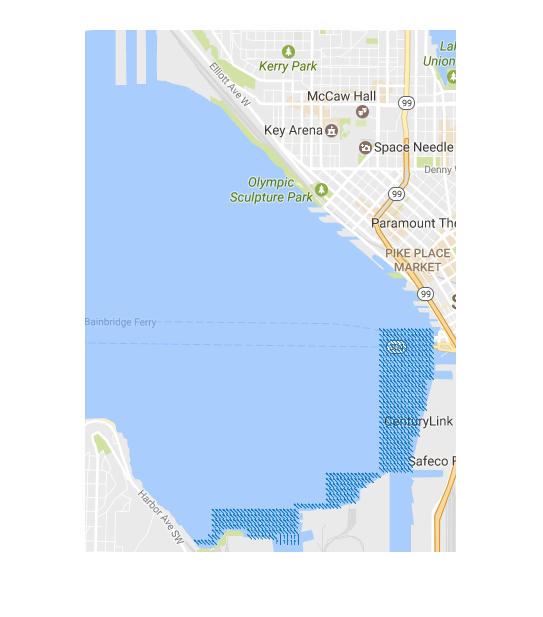
\includegraphics[width=0.4\linewidth]{initialcondnavierstokes.png}
    \caption{Initial Condition for the Navier-Stokes Equations}
    \label{navierstokesinitialcondition}
    %left lower right upper
\end{figure}

%picture here of initial condition
\noindent where the magnitude of each velocity vector at each node $\kappa \in S$ is $3$ meters per second which was chosen arbitrarily. We implement homogeneous Dirichlet conditions along the black boundary shown in Figure \ref{pugetsounddomain} by first considering nodes $i_{N} \in R$ and $\kappa \in S$ where nodes $i_{N}$ also are a part of $\Gamma_{N}$. Now define $\kappa_{x}$, $\kappa_{y}$, $i_{N_{x}}$, $i_{N_{y}}$ as the $x$ and $y$ coordinates of nodes $\kappa$ and $i_{N}$ respectively. If $\abs{\kappa_{x} - i_{N_{x}}} < \epsilon$ and $\abs{\kappa_{y} - i_{N_{y}}} < \epsilon$ for some chosen $\epsilon$, then the velocity vector at node $\kappa$ is $\underline{0}$. We will now develop a finite difference method to approximate the solution to \eqref{navierstokes} at our interior nodes.


\subsection{MacCormack Discretization} \label{MacCormack Section}
Since advective PDEs tend to be unstable when solved for explicitly, we will use a MacCormack method to numerically solve \eqref{navierstokes}. This method uses implicit and explicit Euler steps and takes the average in order to help with stability issues. The MacCormack discretization is a second order accurate method. We begin with the following explicit Euler approximation of the Navier-Stokes equations
\begin{eqnarray}
\frac{\partial v^{f}_{1_{i,j}}}{\partial t} \approx-v^{n}_{1_{i,j}}\frac{\left(v^{n}_{1_{i+1,j}}-v^{n}_{1_{i,j}}\right)}{dx}-v^{n}_{2_{i,j}}\frac{\left(v^{n}_{1_{i,j+1}}-v^{n}_{1_{i,j}}\right)}{dy}+\nu\Delta v^{n}_{1_{CD}}\\
\nonumber
\frac{\partial v^{f}_{2_{i,j}}}{\partial t} \approx -v^{n}_{1_{i,j}}\frac{\left(v^{n}_{2_{i+1,j}}-v^{n}_{2_{i,j}}\right)}{dx}-v^{n}_{2_{i,j}}\frac{\left(v^{n}_{2_{i,j+1}}-v^{n}_{2_{i,j}}\right)}{dy}+\nu\Delta v^{n}_{2_{CD}}\\
\nonumber
\end{eqnarray}

\noindent where $v^{f}_{k_{i,j}}$ denotes the first approximation of the $k$th component of $\underline{v}$ with $k=\{1,2\}$ at spatial nodes $i$, $j$. We also have that $v^{n}_{k_{i,j}}$ is the velocity of the $k$th component of $\underline{v}$ at time-step $n$, $\Delta v^{n}_{k_{CD}}$ is the centered-difference approximation to the Laplacian of the $k$th component of $\underline{v}$ at time step $n$ and $dx$, $dy$ are the spatial steps in the $x$ and $y$ directions respectively. We now calculate our predictive step, $v^{p}_{k_{i,j}}$, with the following


\begin{equation}\label{predictive}
v^{p}_{k_{i,j}}=v^{n}_{k_{i,j}}+\frac{\partial v^{f}_{k_{i,j}}}{\partial t}dt_{FD}
\end{equation}
where $dt_{FD}$ is the time-step of our finite difference method. Using this predictive step, we now calculate our second approximations to \eqref{navierstokes}, $\frac{\partial v^{s}_{k_{i,j}}}{\partial t}$, with the following

\begin{eqnarray}
\frac{\partial v^{s}_{1_{i,j}}}{\partial t} \approx \left(-v^{f}_{1_{i,j}}\frac{\left(v^{f}_{1_{i,j}}-v^{f}_{1_{i-1,j}}\right)}{dx}-v^{f}_{2_{i,j}}\frac{\left(v^{f}_{1_{i,j}}-v^{f}_{1_{i,j-1}}\right)}{dy}+\nu\Delta v^{f}_{1_{CD}}\right)\\
\nonumber
\frac{\partial v^{s}_{2_{i,j}}}{\partial t} \approx \left(-v^{f}_{1_{i,j}}\frac{\left(v^{f}_{2_{i,j}}-v^{f}_{2_{i-1,j}}\right)}{dx}-v^{f}_{2_{i,j}}\frac{\left(v^{n}_{2_{i,j}}-v^{f}_{2_{i,j-1}}\right)}{dy}+\nu\Delta v^{f}_{2_{CD}}\right).\\
\nonumber
\end{eqnarray}
Using this second approximation to \eqref{navierstokes}, we now calculate our next time-step approximations, $v^{n+1}_{k_{i,j}}$, with

\begin{equation}\label{fullstep}
v^{n+1}_{k_{i,j}}=v^{n}_{k_{i,j}}+\left(\frac{\partial v^{f}_{k_{i,j}}}{\partial t}+\frac{\partial v^{s}_{k_{i,j}}}{\partial t}\right)\frac{dt_{FD}}{2}.
\end{equation}

\noindent Using this MacCormack method, we now are able to run our code until we obtain the steady state of $\underline{v}$ which can be found in figure \ref{navierstokessteadystate}.

%figure of steady state here
\begin{figure}[H]  
\centering   
   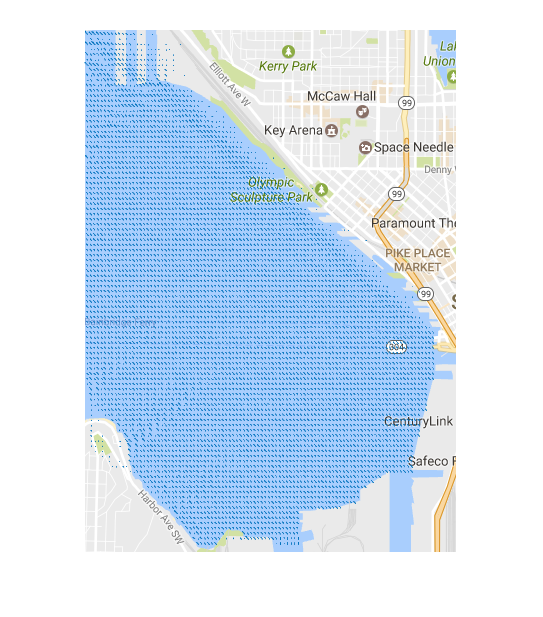
\includegraphics[width=0.4\linewidth]{navierstokessteadystate.png}
    \caption{Steady State Solution to the Navier-Stokes Equations}
    \label{navierstokessteadystate}
    %left lower right upper
\end{figure}

Our tolerance scheme failed in within our domain in the upper left hand corner as shown in Figure \ref{navierstokessteadystate}
however, we are not concerned with this as we are not concerned with modeling contaminant flow in that portion of the domain. The tolerance scheme also failed slightly in the lower-left hand portion of our domain. This is an error that we would like to improve on in the future by increasing $\epsilon$ slightly.


\section{Results} \label{Results Section}
%Explain running two models
Using our finite element method and MacCormack discretization, we are now able to create our models of contaminant flow. We will have two models where the first will model point source contaminant flow in $\Omega$ while that second will model a constant spill pouring into the domain from a collection of nodes in $\Gamma_{\texttt{N $\rightarrow$ D}}$. For stability purposes, we will utilize a diffusivity of $1$ square meter per second in our models. We take our velocity vector field and divide each term in it by $10$ for stability reasons. This diffusivity and velocity vector field are not realistic and we want to fix these stability issues in the future so that we can use a realistic diffusivity and magnitude of velocity for our velocity vector field.

\subsection{Point Source Model}
We begin with modeling point source contaminant flow in our domain shown in Figure \ref{pugetsounddomain} which will model a sinking ship. The following series of snap-shots show the progression of contaminant flow at different times $t$

\begin{figure}[H]
   
\centering   
   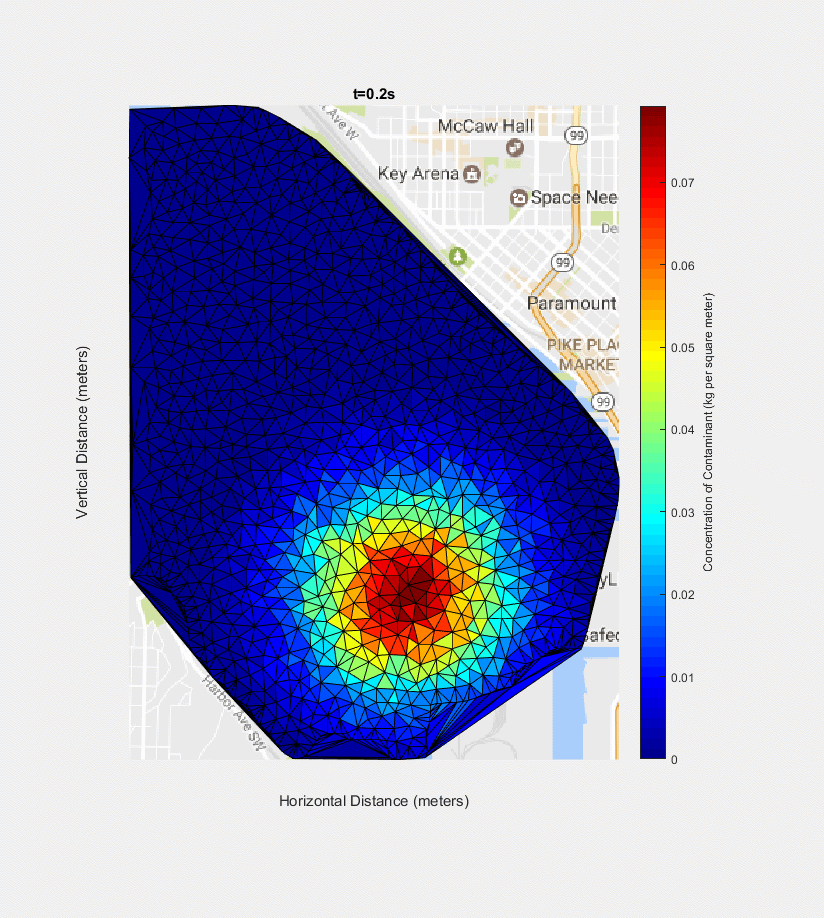
\includegraphics[trim=0mm 0mm 0mm 0mm,clip,width=0.5\linewidth]{point1.png}
    \caption{Point Source Numerical Solution at time $t = 0.2$ seconds}
    \label{Results.2secondspoint}
\end{figure}

\begin{figure}[H]
   
\centering   
   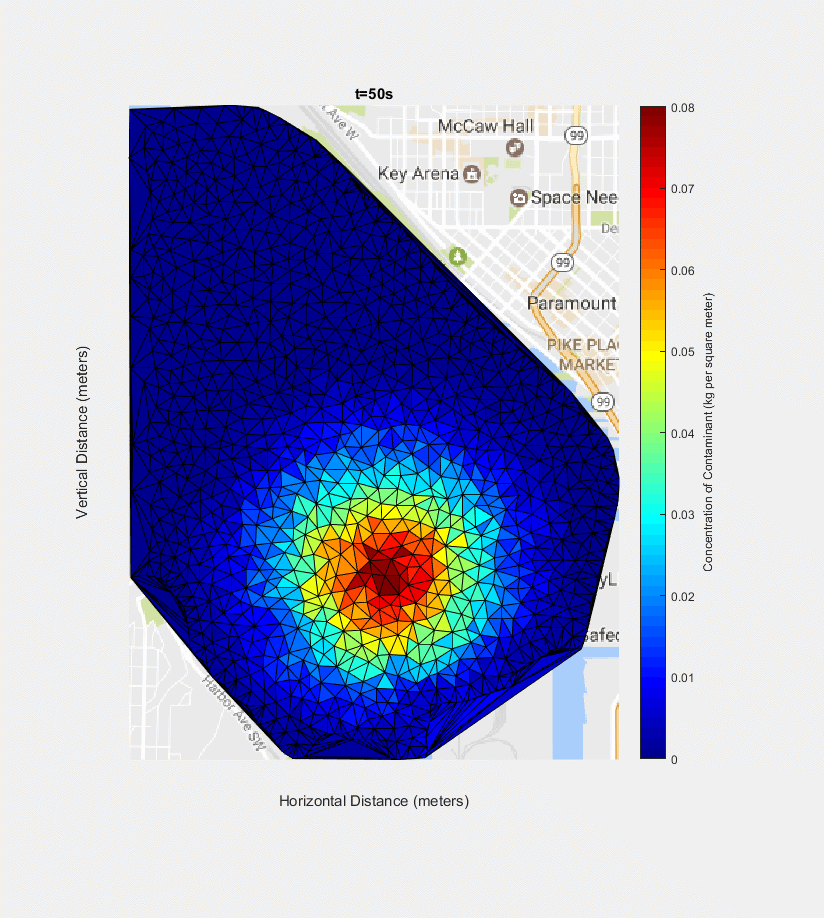
\includegraphics[trim=0mm 0mm 0mm 0mm,clip,width=0.5\linewidth]{point2.png}
    \caption{Point Source Numerical Solution at time $t = 50$ seconds}
    \label{Results50secondspoint}
\end{figure}

\begin{figure}[H]
   
\centering   
   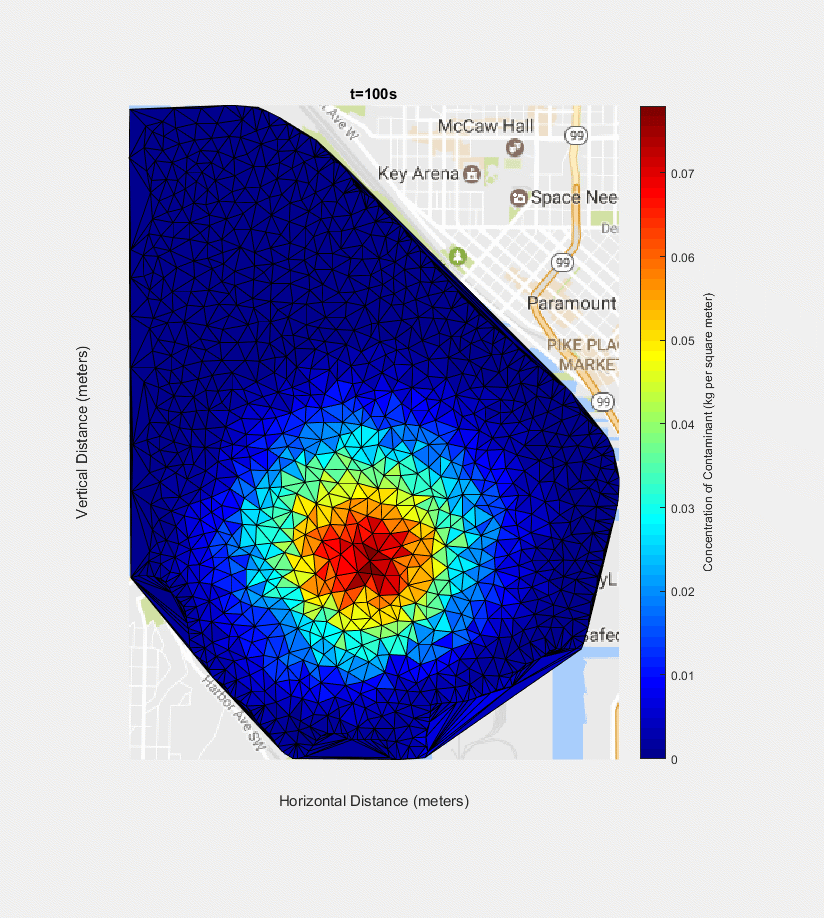
\includegraphics[trim=0mm 0mm 0mm 0mm,clip,width=0.5\linewidth]{point3.png}
    \caption{Point Source Numerical Solution at time $t = 100$ seconds}
    \label{Results100secondspoint}
\end{figure}

\begin{figure}[H]
   
\centering   
   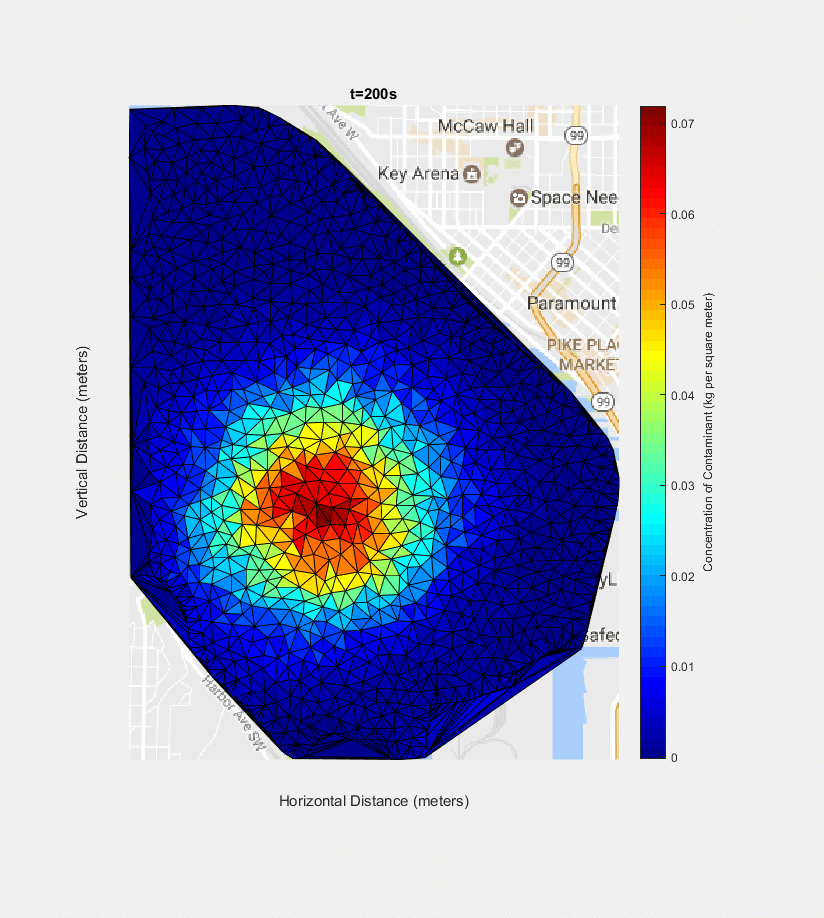
\includegraphics[trim=0mm 0mm 0mm 0mm,clip,width=0.5\linewidth]{point4.png}
    \caption{Point Source Numerical Solution at time $t = 200$ seconds}
    \label{Results200secondspoint}
\end{figure}

\begin{figure}[H]
\centering   
  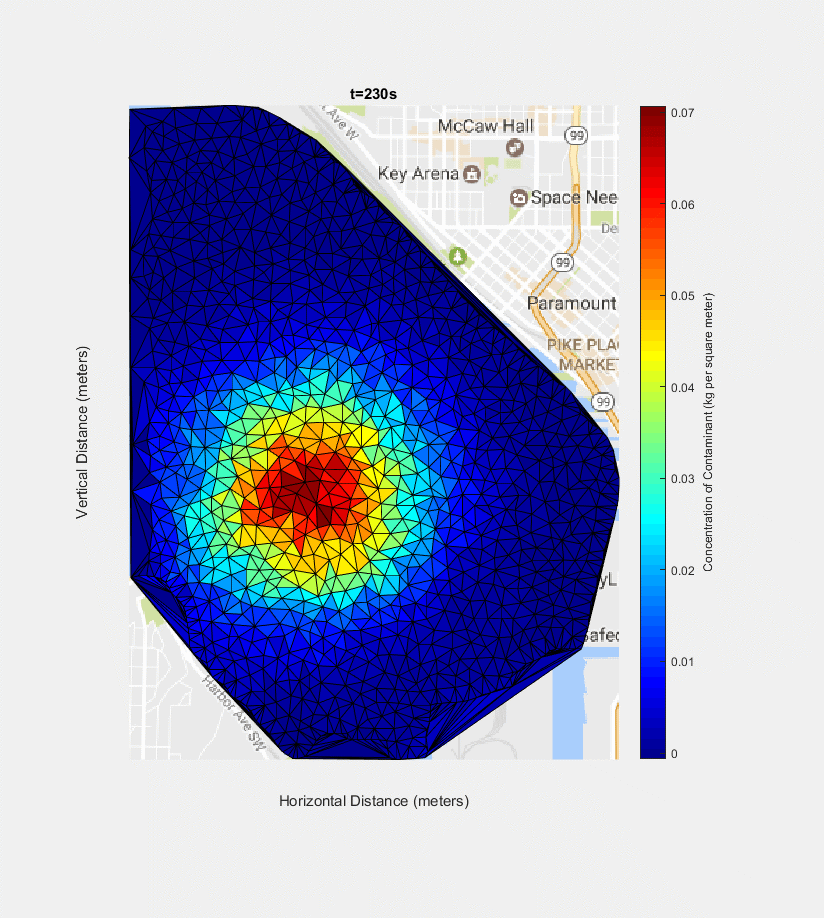
\includegraphics[trim=0mm 0mm 0mm 0mm,clip,width=0.5\linewidth]{point5.png}
   \caption{Point Source Numerical Solution at time $t = 230$ seconds}
   \label{Results230secondspoint}
\end{figure}


\noindent In order to confirm our numerical results we will need to test for the convergence of our numerical solution as well as conservation of concentration since we are not adding or subtracting any contaminant in this first model.


\subsection{Convergence Testing for Point Source Model} \label{ConvergencePointModelSection}
In order to perform convergence testing, we will run our point source model code for a $230$ seconds of simulated time and then save the resulting final numerical solution into a vector. We will do this starting with $dt=0.1$ and then we will decrease $dt$ by a factor of $10$ each time we run the code and save the final result. We will then measure the Euclidean distance between final result vectors as expressed by

\begin{equation} \label{convergencetest}
\left|\left| \underline{U}^{end}_{dt_{1}}-\underline{U}^{end}_{dt_{2}} \right|\right|
\end{equation}

\noindent where $\underline{U}^{end}_{dt_{1}}$ is the numerical solution using a time-step of $dt_{1}$ at the final time of $t=230$ seconds while $\underline{U}^{end}_{dt_{2}}$ is similar in notation except this solution uses a time-step of $dt_{2}$ which is $10$ times smaller than $dt_{1}$. Our solution converges, if each time we decrease $dt$ by a factor of $10$, then the Euclidean distance between numerical solutions at the final time should decrease by a factor of $10$ as well. When we test this, we get the following table.

\begin{table}[H]
\centering
\caption{Convergence Testing for Point Source Model}
\label{convergencemodelpoint}
\begin{tabular}{|l|l|}
\hline
Time-Steps           & Euclidean Distance Between Numerical Solutions \\ \hline
$0.1$ and $0.01$     & $3.3623 \times 10^{-4}$              \\ \hline
$0.01$ and $0.001$   & $3.3656 \times 10^{-5}$              \\ \hline
$0.001$ and $0.0001$ & $3.3660 \times 10^{-6}$                                    \\ \hline
\end{tabular}
\end{table}

\noindent We see from Table \ref{convergencemodelpoint}, our numerical solution converges as we decrease $dt$ by a factor of $10$. We also want to test conservation of concentration of contaminant.


\subsection{Conservation of Concentration for Point Source Model} \label{ConservationPointModelSection}
Since we are not adding or subtracting any concentration of contaminant in our point source model, contaminant should be conserved. Therefore, we will sum the total concentration of contaminant at each time-step in our numerical solution and plot it to see if there's any significant change in concentration of contaminant. When we do this, we obtain Figure \ref{conservationofconcentrationofcontaminant}.

\begin{figure}[H]   
\centering   
   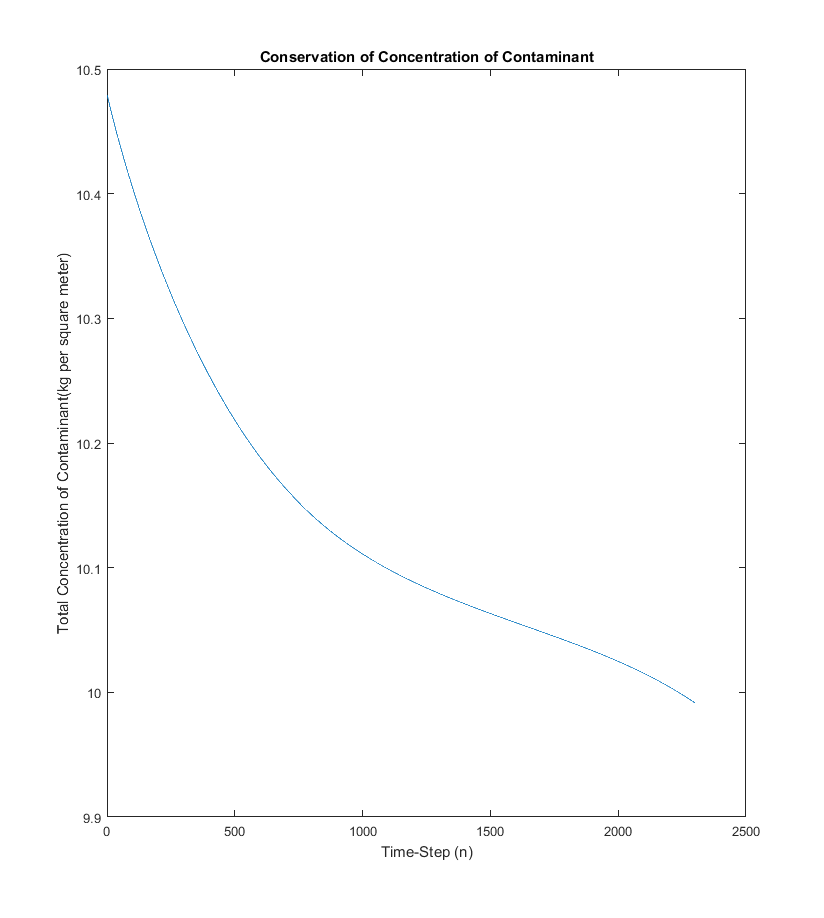
\includegraphics[trim=0mm 0mm 0mm 0mm,clip,width=0.5\linewidth]{pointconservation.png}
    \caption{Conservation of Concentration of Contaminant}
    \label{conservationofconcentrationofcontaminant}
\end{figure}

As we see in Figure \ref{conservationofconcentrationofcontaminant}, the concentration of contaminant is not fully conserved. We will now check the rate as to how fast we are losing contaminant as time carries on so we employ a centered-difference numerical differentiation scheme which is a second order accurate method in order to find the derivative of the vector shown in Figure \ref{conservationofconcentrationofcontaminant}. When we do this, we obtain Figure \ref{derivcons} which shows the rate of change of contaminant in $\Omega$.


\begin{figure}[H]   
\centering   
   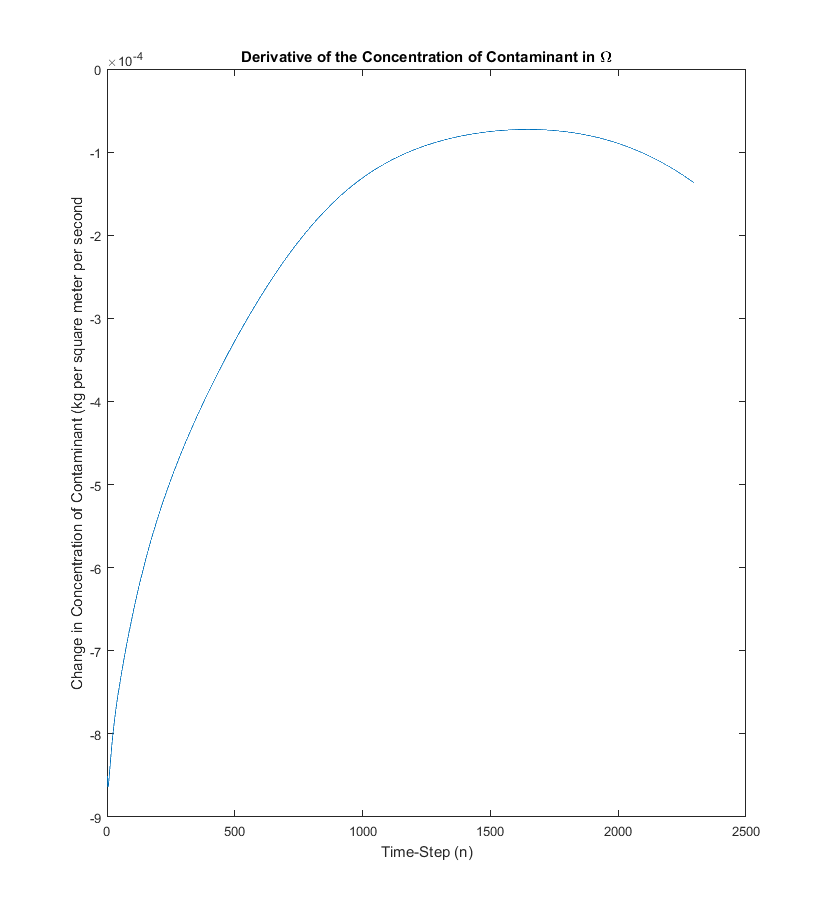
\includegraphics[trim=0mm 0mm 0mm 0mm,clip,width=0.5\linewidth]{derivconservation.png}
    \caption{Rate of Change of Concentration of Contaminant in $\Omega$}
    \label{derivcons}
\end{figure}

As we see, the rate of decrease of contaminant is small for the $230$ seconds of simulation time that we ran our program for. A reason for this decrease in contaminant could be the fact that we use a barycentric approximation of each triangular element that forms each basis function. We would remedy this problem by increasing our number of nodes $N$ and improving the approximations used to derive each mass matrix and the right-hand side. We could also employ a finite volume method to fix this issue.
\subsection{Constant Source Model} \label{ConstantSourceModelSection}
Using the same diffusivity of $1$ square meter per second and velocity vector field which was found using an initial magnitude of velocity of $3$ meters per second as before, we will now model contaminant flow from a constant source along our boundary as shown in magenta in Figure \ref{pugetsounddomain2}. We will add a constant amount of concentration of contaminant into our domain each time-step so we expect linear growth in the concentration of contaminant as time increases. The following images show the contaminant flow for this situation when we run our program for $560$ seconds of simulation time. You'll find that the solution goes heavily unstable as it runs but then as time continues on, the diffusive term takes over and the solution stabilizes.

\begin{figure}[H]   
\centering   
   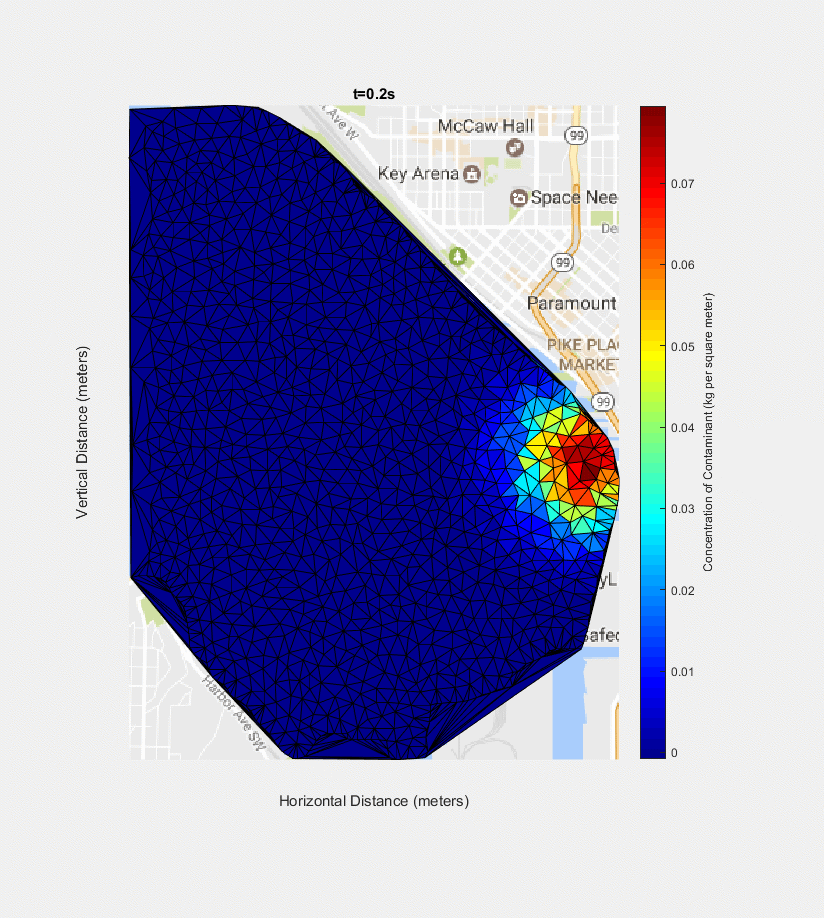
\includegraphics[trim=0mm 0mm 0mm 0mm,clip,width=0.5\linewidth]{const1.png}
    \caption{Constant Source Numerical Solution at $t=0.2$ seconds}
    \label{constant0.2seconds}
\end{figure}

\begin{figure}[H]   
\centering   
   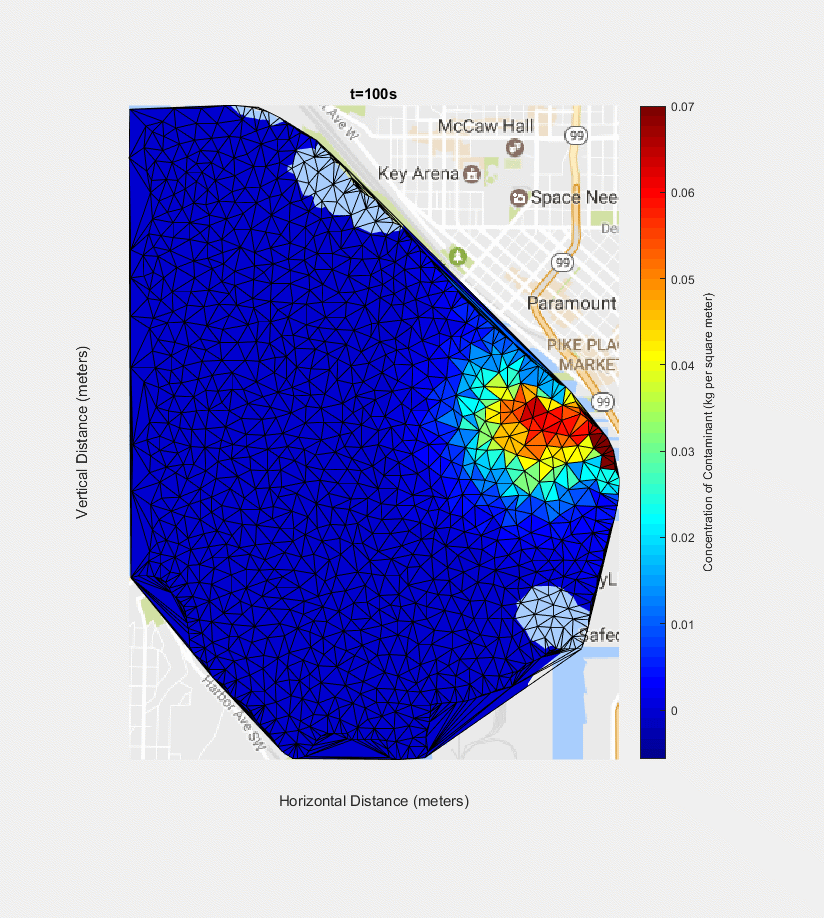
\includegraphics[trim=0mm 0mm 0mm 0mm,clip,width=0.5\linewidth]{const2.png}
    \caption{Constant Source Numerical Solution at $t=100$ seconds}
    \label{constant100seconds}
\end{figure}


\begin{figure}[H]   
\centering   
   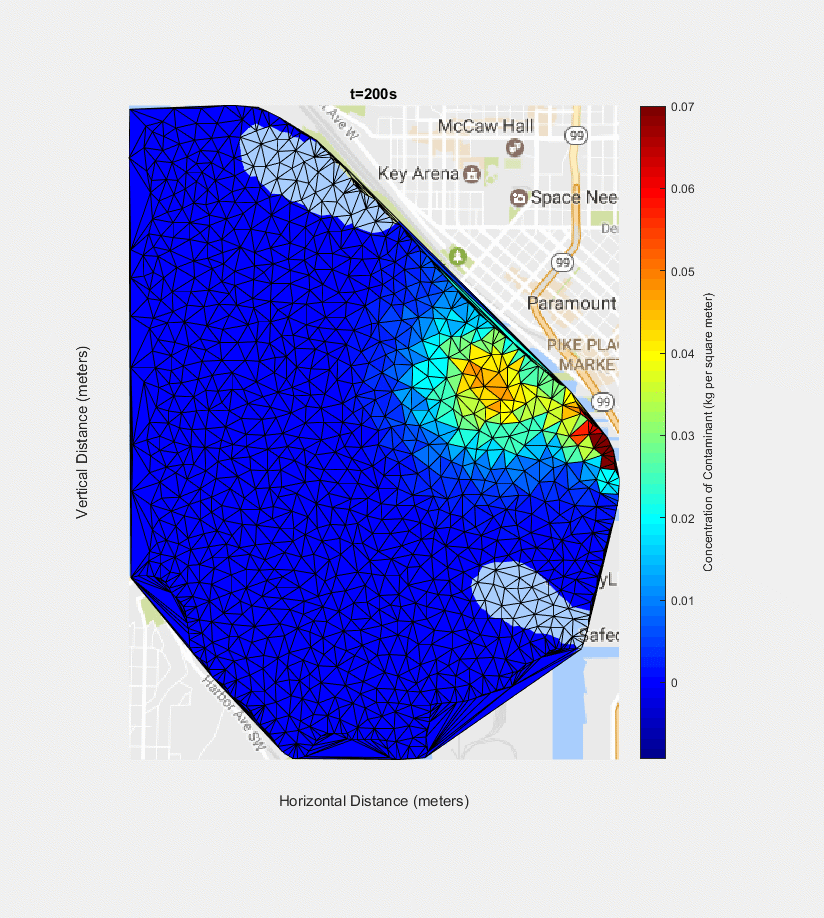
\includegraphics[trim=0mm 0mm 0mm 0mm,clip,width=0.5\linewidth]{const3.png}
    \caption{Constant Source Numerical Solution at $t=200$ seconds}
    \label{constant200seconds}
\end{figure}


\begin{figure}[H]   
\centering   
   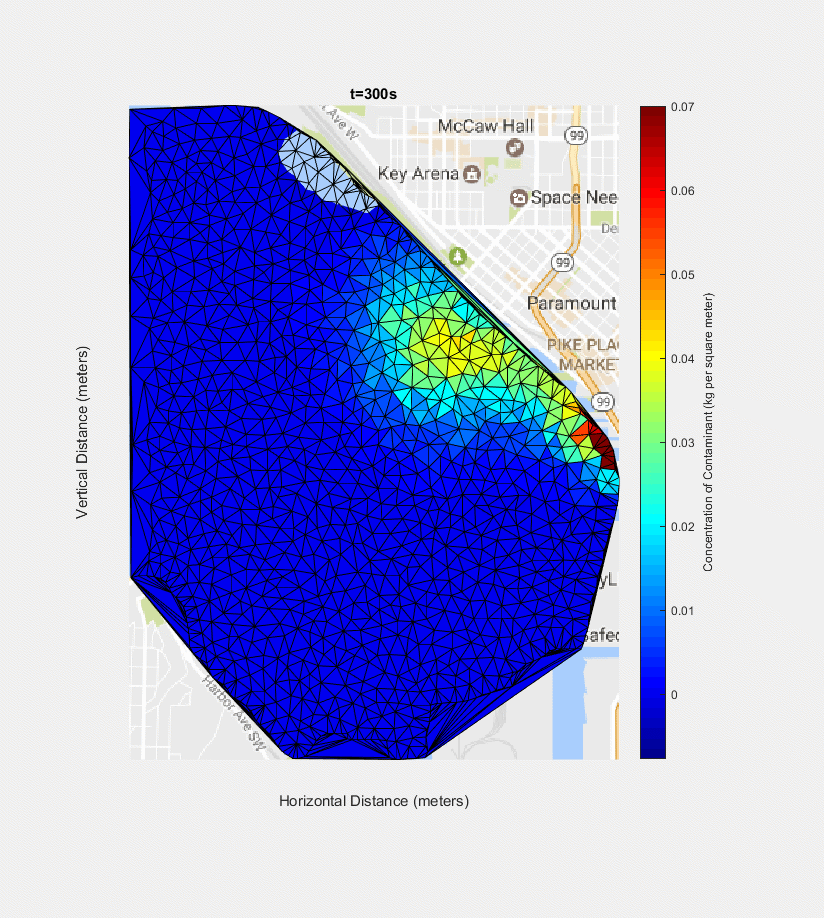
\includegraphics[trim=0mm 0mm 0mm 0mm,clip,width=0.5\linewidth]{const4.png}
    \caption{Constant Source Numerical Solution at $t=300$ seconds}
    \label{constant300seconds}
\end{figure}

\begin{figure}[H]   
\centering   
   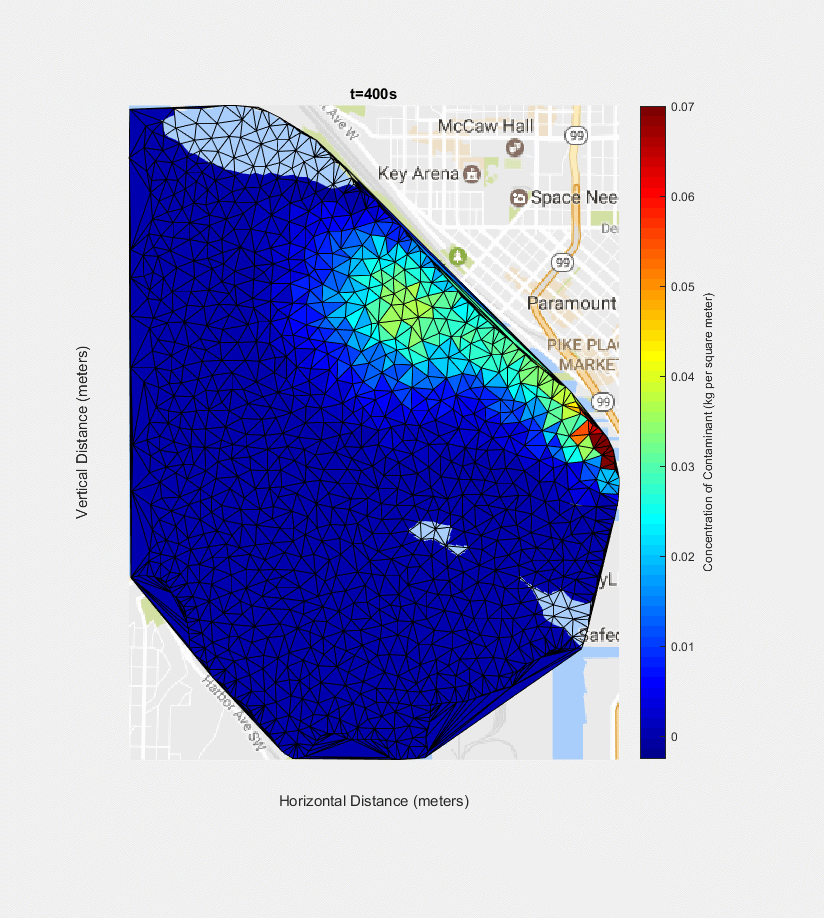
\includegraphics[trim=0mm 0mm 0mm 0mm,clip,width=0.5\linewidth]{const5.png}
    \caption{Constant Source Numerical Solution at $t=400$ seconds}
    \label{constant400seconds}
\end{figure}

\begin{figure}[H]   
\centering   
   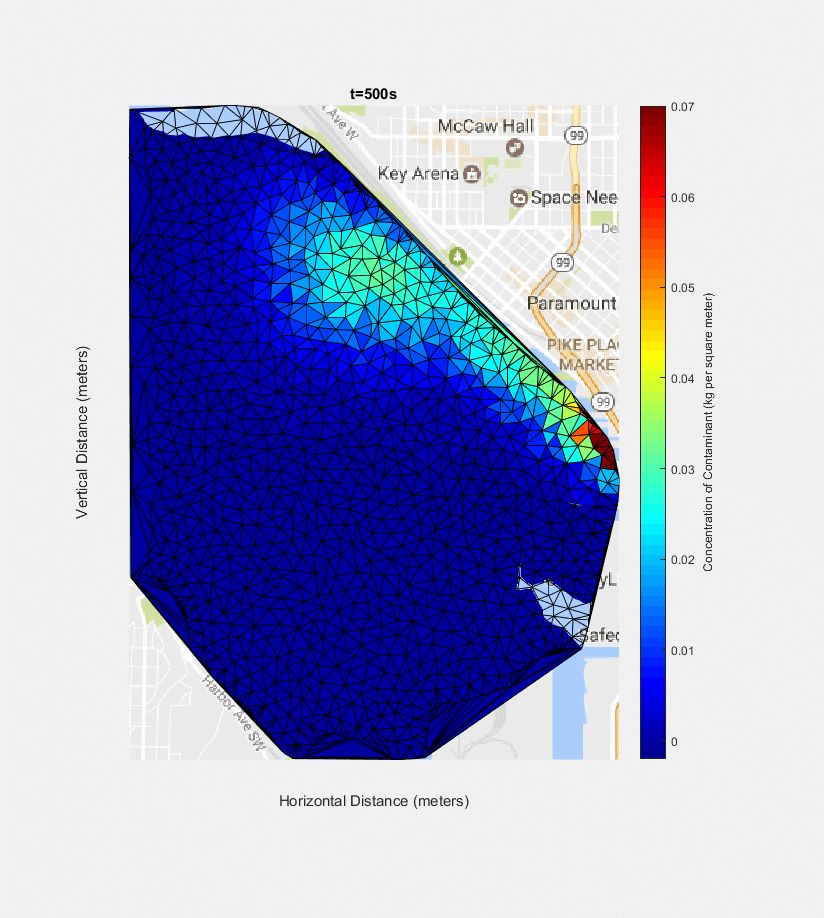
\includegraphics[trim=0mm 0mm 0mm 0mm,clip,width=0.5\linewidth]{const6.png}
    \caption{Constant Source Numerical Solution at $t=500$ seconds}
    \label{constant500seconds}
\end{figure}



\begin{figure}[H]   
\centering   
   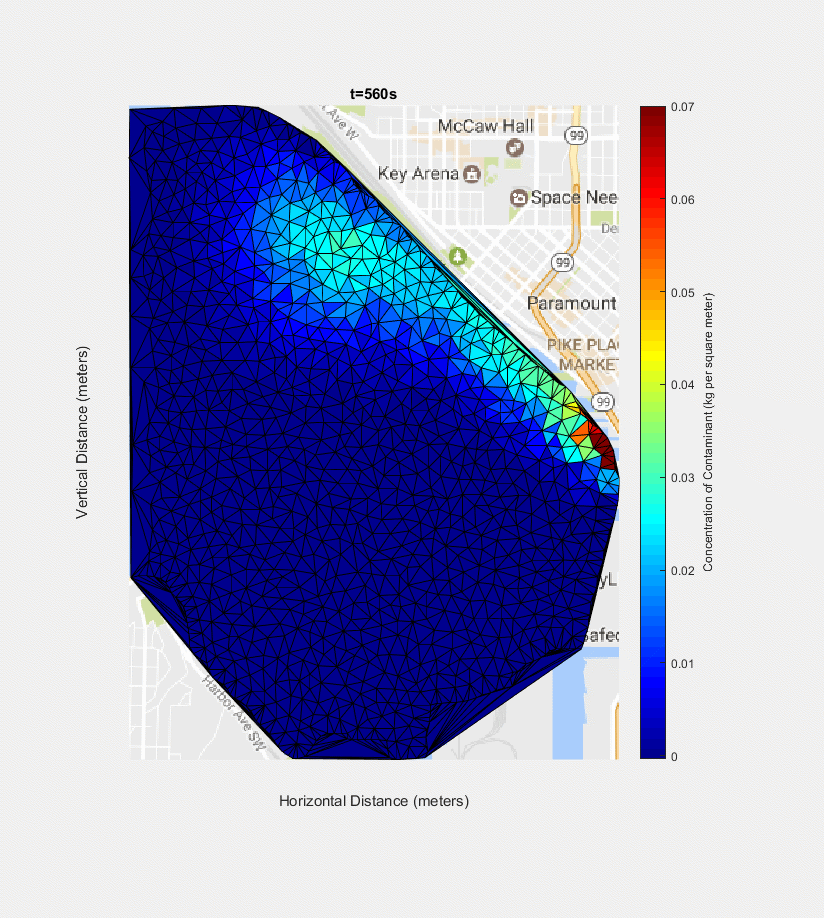
\includegraphics[trim=0mm 0mm 0mm 0mm,clip,width=0.5\linewidth]{const7.png}
    \caption{Constant Source Numerical Solution at $t=560$ seconds}
    \label{constant560seconds}
\end{figure}

Even though we have stability issues as the simulation continues, we find that we eventually reach useful results. As was the case with our point source model, we will test this model for convergence and instead of conservation (since in this case we are adding in contaminant to our domain) we will test for linear addition of concentration of contaminant.


\subsection{Convergence Testing Constant Source Model} \label{ConvergenceConstantModelSection}
We use the same method for testing convergence in this case as we did when we tested for convergence in our point source model to obtain Table \ref{convergencemodelconstant}.

\begin{table}[H]
\centering
\caption{Convergence Testing for Constant Source Model}
\label{convergencemodelconstant}
\begin{tabular}{|l|l|}
\hline
Time-Steps           & Euclidean Distance Between Numerical Solutions \\ \hline
$0.1$ and $0.01$     & $2.8178 \times 10^{-4}$              \\ \hline
$0.01$ and $0.001$   & $2.8262 \times 10^{-5}$              \\ \hline
$0.001$ and $0.0001$ & $2.8271 \times 10^{-6}$                                      \\ \hline
\end{tabular}
\end{table}

\noindent As we see in Table \ref{convergencemodelconstant}, our numerical solution converges. We will now test for addition of concentration of contaminant into our domain.

\subsection{Conservation of Concentration for Constant Source Model} \label{IncreaseConstantModelSection}
We test for addition of concentration of contaminant into our domain using the same methods as described before with our point source model. In this case, we expect to see a linear growth in the concentration of contaminant since the rate at which we add contaminant into our domain is constant. When we test this, we obtain Figure \ref{constantaddition}.

\begin{figure}[H]   
\centering   
   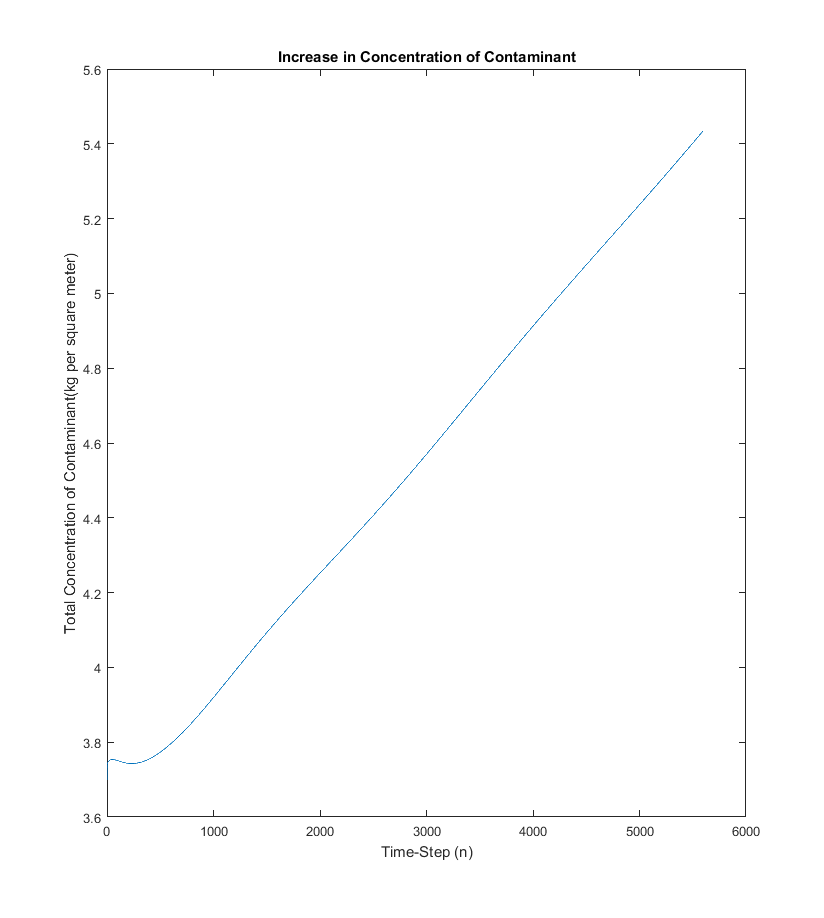
\includegraphics[trim=0mm 0mm 0mm 0mm,clip,width=0.5\linewidth]{constincrease.png}
    \caption{Addition of Concentration of Contaminant in $\Omega$}
    \label{constantaddition}
\end{figure}

We see in Figure \ref{constantaddition} that as time increases, the total concentration of contaminant in $\Omega$ linearly increases. Using a diffusivity of $D=1$ square meter per second, our velocity vector steady state shown in Figure \ref{navierstokessteadystate} scaled down, and our domain shown in Figure \ref{pugetsounddomain2}, we were able to create a numerical approximation to the solution of \eqref{advecdiff}. Using these parameters, to show that our numerical solution modeling a constant source spill converges and we obtain acceptable results for the addition of concentration of contaminant. We will now test the sensitivity of our numerical solutions to $D$.


\section{Sensitivity Analysis} \label{SensitivityAnalysisSection}
We test the sensitivity of our numerical results to $D$ by first selecting a set of nodes $i \in R$ such that $145 < i_{x} <155$ where $i_{x}$ is the $x$ coordinate of node $i$. Each node that is a part of this region is circled in Figure \ref{sensewall}.

\begin{figure}[H]   
\centering   
   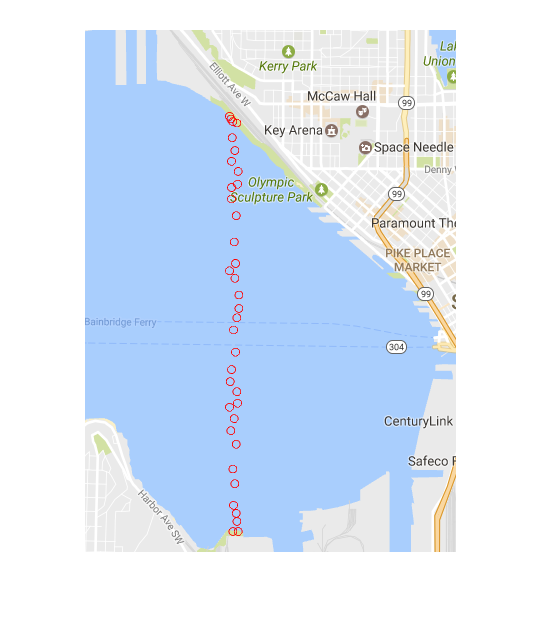
\includegraphics[trim=0mm 0mm 0mm 0mm,clip,width=0.5\linewidth]{sensewall.png}
    \caption{Region Used to Measure Sensitivity of Solutions}
    \label{sensewall}
\end{figure}

\noindent We will measure the amount total of contaminant that flows through this region at each time-step.
\subsection{Sensitivity Analysis of Point Source Model} \label{SensitivityAnalysisPointSourceSection}
We start with a sensitivity analysis of our point source model. We use the above mentioned method and we obtain the  Figure \ref{sensepoint}.
\begin{figure}[H]   
\centering   
   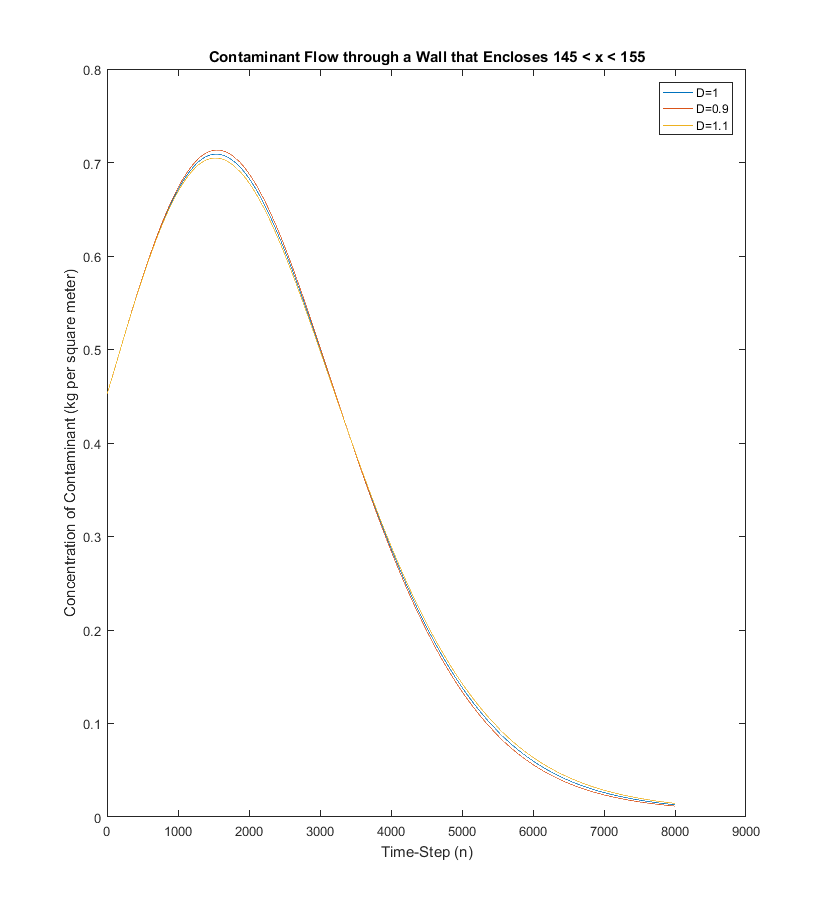
\includegraphics[trim=0mm 0mm 0mm 0mm,clip,width=0.5\linewidth]{sensepoint.png}
    \caption{Difference in Numerical Solutions at Different Diffusivities}
    \label{sensepoint}
\end{figure}


\noindent As we see, there is very little graphical difference between solutions by varying $D$ by $\pm 10\%$. We will now perform a numerical sensitivity analysis of these results using the following

\begin{equation}
S=\frac{\Delta x D}{x \Delta D}
\end{equation}

\noindent where $\Delta x$ is the change in concentration of contaminant between solutions when $D=1$ and $D=1.1$ or $D=0.9$, $\Delta D$ is the change in diffusivity, and $x$ is the concentration of contaminant when $D=1.1$ or $D=0.9$. We will look at the sensitivity at the time-step where the most concentration of contaminant is present in our region. This appears to be roughly w $n \approx 1900$ so we will measure the sensitivity of our model to $\pm 10\%$ of diffusivity at time-step $n=1900$. When we we do this we obtain the following table.


\begin{table}[H]
\centering
\caption{Sensitivity Point Source Model}
\label{sensitivitymodel1}
\begin{tabular}{|l|l|}
\hline
Change in Diffusivity           & $S$ \\ \hline
$+10\%$    & $-0.0773$              \\ \hline
$-10\%$   & $0.0646$              \\ \hline
\end{tabular}
\end{table}
\noindent As we see, our point source model is not sensitive to small changes in $D$.


\subsection{Sensitivity Analysis Constant Source Model}  \label{SensitivityAnalysisConstantSourceSection}
We will now repeat the same process mentioned in the previous subsection for our constant source model. When we do this, we obtain the following figure.

\begin{figure}[H]   
\centering   
   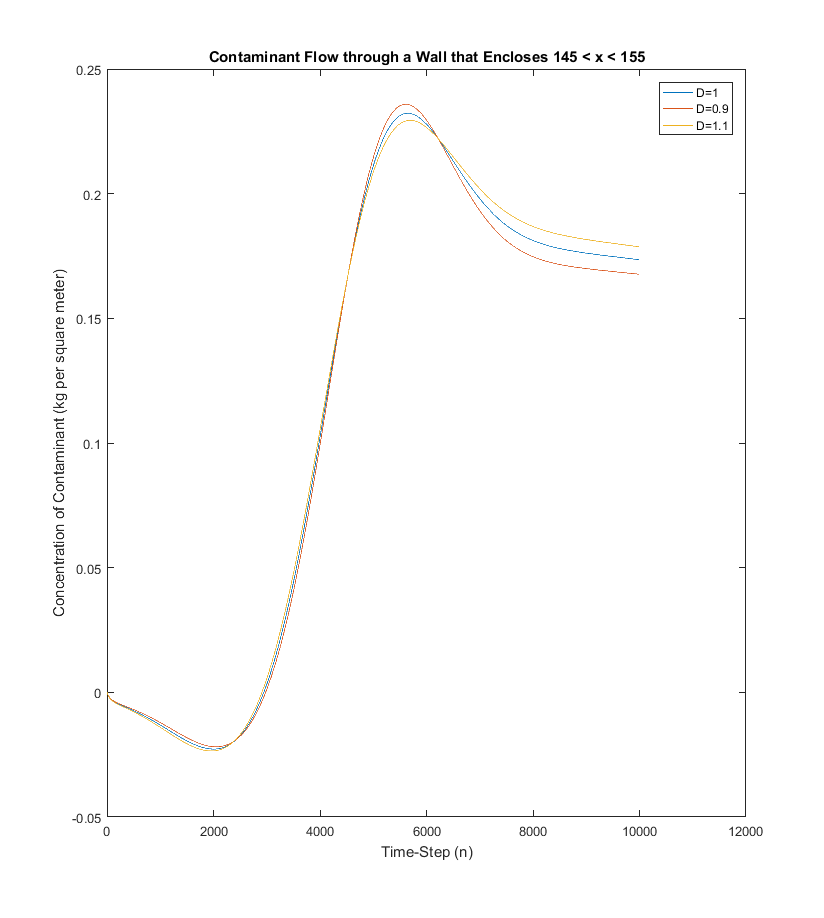
\includegraphics[trim=0mm 0mm 0mm 0mm,clip,width=0.5\linewidth]{senseconst.png}
    \caption{Difference in Numerical Solutions at Different Diffusivities}
    \label{senseconst}
\end{figure}

Graphically, our constant source model appears to be more sensitive than our point source model. We repeat our numerical sensitivity analysis of our constant source model at time-step $n=5900$ and we obtain the following table.

\begin{table}[H]
\centering
\caption{Sensitivity Constant Source Model}
\label{sensitivitymodel2}
\begin{tabular}{|l|l|}
\hline
Change in Diffusivity           & $S$ \\ \hline
$+10\%$    & $-0.0893$              \\ \hline
$-10\%$   & $0.0870$              \\ \hline
\end{tabular}
\end{table}

\noindent As we see, our constant source model is slightly more sensitive to changes in $D$ than our point source model however, it is largely still insensitive to changes in $D$.

\section{Future Work} \label{futureworksection}
The first issue that needs to be address is the stability problem. In order to help fix this problem we would implement optimized meshing software to maximize the number of nodes we use in our finite element code. The next way we could improve on the stability issue is to find a way to avoid using a barycentric approximation of the basis functions when we build our mass matrices and right-hand side. After fixing the stability issue, we would then use a realistic diffusivity and magnitude for our velocity vector field. Finally, we want to refine our tolerance scheme which we use to connect our finite element and finite difference code.

\section{Conclusion} \label{conclusionsection}
Contaminant spills in aquatic ecosystems cause immense damage to the environment. The goal of this paper was to expand on research that has already been done in order to mathematically predict how to most efficiently clean up a spill, if one were to occur in a body of water as well as find out what areas of that ecosystem would experience the most damage. In this paper, we were able to give an overview of the finite element method, numerically solve the advection-diffusion equation and Navier-Stokes equations on a Puget Sound domain, offer results, and provide sensitivity analyses of our results. Using the ideas presented in this paper and in section \ref{futureworksection}, we will be able to extend on the this work to better model contaminant flow in bodies of water.
\newpage
\section{Works Cited}
\begin{thebibliography}{3}
\bibitem{50LinesofMATLAB}
\textit{Remarks around 50 lines of Matlab: short finite element implementation}, Jochen Alberty, Carsten Carstensen and Stefan A. Funken, \textit{Numerical Algorithms 20} (1999), pp. 117-137

\bibitem{Johnson}
\textit{Numerical Solution of Partial Differential Equations by the Finite Element Method}, Claes Johnson, Dover Publications, INC. Mineola, New York (2009) pp. 14-20

%\bibitem{DiffusivityCoefficientat22degrees}
%\textit{Modeling the BP Oil Spill of 2010: A Simplified Model of Oil Diffusion in Water}, Eilleen Ao-leong, Anna Chang, Steven Gu, \textit{BENG 221 - Fall 2012} (2012) pp. 4

%\bibitem{Kinematic Viscosity of Water at 22 degrees}
%http://www.viscopedia.com/viscosity-tables/substances/water/

\bibitem{Sullivan}
Dr. Eric Sullivan, Assistant Professor of Mathematics, Carroll College (2017)

\end{thebibliography}

\end{document}
    
    






       